% !TEX TS-program = pdflatex
% !TEX encoding = UTF-8 Unicode

% This is a simple template for a LaTeX document using the "article" class.
% See "book", "report", "letter" for other types of document.

\documentclass[11pt]{article} % use larger type; default would be 10pt

\usepackage[utf8]{inputenc} % set input encoding (not needed with XeLaTeX)

%%% Examples of Article customizations
% These packages are optional, depending whether you want the features they provide.
% See the LaTeX Companion or other references for full information.

%%% PAGE DIMENSIONS
\usepackage{geometry} % to change the page dimensions
\geometry{a4paper} % or letterpaper (US) or a5paper or....
% \geometry{margin=2in} % for example, change the margins to 2 inches all round
% \geometry{landscape} % set up the page for landscape
%   read geometry.pdf for detailed page layout information

\usepackage{graphicx} % support the \includegraphics command and options

% \usepackage[parfill]{parskip} % Activate to begin paragraphs with an empty line rather than an indent

%%% PACKAGES
\usepackage{booktabs} % for much better looking tables
\usepackage{array} % for better arrays (eg matrices) in maths
%\usepackage{paralist} % very flexible & customisable lists (eg. enumerate/itemize, etc.)
\usepackage{verbatim} % adds environment for commenting out blocks of text & for better verbatim
\usepackage{subfig} % make it possible to include more than one captioned figure/table in a single float
\usepackage{setspace} %paquete para interlineado
\usepackage{graphicx} %para insertar graficos
\usepackage{parskip} % npi de q es
\usepackage{color} %colores


% These packages are all incorporated in the memoir class to one degree or another...

%%% HEADERS & FOOTERS
\usepackage{fancyhdr} % This should be set AFTER setting up the page geometry
\pagestyle{fancy} % options: empty , plain , fancy
\renewcommand{\headrulewidth}{0pt} % customise the layout...
\lhead{}\chead{}\rhead{}
\lfoot{}\cfoot{\thepage}\rfoot{}

%%% SECTION TITLE APPEARANCE
\usepackage{sectsty}
\allsectionsfont{\sffamily\mdseries\upshape} % (See the fntguide.pdf for font help)
% (This matches ConTeXt defaults)

%%% ToC (table of contents) APPEARANCE
\usepackage[nottoc,notlof,notlot]{tocbibind} % Put the bibliography in the ToC
\usepackage{color}
\usepackage[titles,subfigure]{tocloft} % Alter the style of the Table of Contents
\renewcommand{\cftsecfont}{\rmfamily\mdseries\upshape}
\renewcommand{\cftsecpagefont}{\rmfamily\mdseries\upshape} % No bold!

%%% END Article customizations

\usepackage[spanish]{babel}
\usepackage{listings} 
%%% The "real" document content comes below...

\title{Investigación de Lenguajes - HTML}
<<<<<<< HEAD
\author{Angel Gonzalez\\ Fausto Mora\\Christian Vergara}
=======
\author{Fausto Mora\\ Christian Vergara \\ Angel Gonzalez}
\begin{document}
\author{Javier Tibau}
>>>>>>> c83f37ea927560365018cb841d502836f3e8957a
%\date{} % Activate to display a given date or no date (if empty),
         % otherwise the current date is printed 

\maketitle
%\tableofcontents % No hace falta un TOC en un artículo corto

\section{Introducción}
\newcommand{\oops}[1]{\textit{#1}}

\noindent \emph{HTML \oops{{\color{black}Hyper Text Markup Language}}}, es un lenguaje utilizado para crear páginas web, con el se escriben muchas de las estructuras de sitios que existen actualmente en internet.
Los programadores utilizan el lenguaje HTML para crear sus páginas web, estos utilizan programas que generan sitios escritos en este lenguaje y los navegadores que utilizamos a diario muestran las páginas web después de interpretar su contenido HTML.\\

\noindent El lenguaje HTML fue estandarizado por el organismo W3C (\oops{World Wide Web Consortium}) el cual define un estándar para todas las empresas relacionadas con el uso del internet. De esta manera el lenguaje HTML es un lenguaje universalmente reconocido y el cual permite publicar información de manera global.\\

\noindent El eje principal de HTML es la \oops{referenciación} , es decir, para insertar contenido multimedia como fotos, música, videos, archivos, etc , estos no van dentro del código de la página, sino que se hace referencia a los mismos que se encuentran en una ubicación externa. El navegador que interpreta el código HTML une todos estos archivos mostrando así, una página final, mientras que el proceso de creación del código HTML contiene unicamente texto. Ya que éste es un lenguaje estandar es necesario que todos los navegadores ejecuten de la misma manera el código.\\

\noindent A lo largo del desarrollo de HTML, éste ha incorporado diferentes características para adaptarlo a nuevas plataformas (smartphones, tablet, etc), Estos cambios son añadidos a los navegadores cada vez que estos lanzan una nueva versión o actualización. Para la correcta interpretación de una nueva versión de HTML es necesario que los navegadores esten actualizados. Por el contrario las versiones actuales de navegadores por lo general mantienen la interpretación de versiones anteriores de HTML, para poder visualizar el contenido de aplicaciones desarrolladas por las mismas, aunque la apariencia no sea moderna.\\



\section{Características}
\section{Historia}
\section{Tutorial de Instalación}
Para escribir HTML lo único que se necesita es un editor de texto ASCII, como EDIT del MS-DOS o el Bloc de notas de Windows. \singlespace
\thinspace Existen una serie de programas que ayudan en la elaboración de documentos HTML, como HTMLED (shareware) o HTML Assistant, ambos para Windows, pero no son imprescindibles para escribir el código. Lo que si es necesario es un programa cliente WWW, tal como Mosaic, o Netscape, para probar el documento a medida que lo vamos desarrollando.

\section{Ejemplos del Codigo:}


En la imagen (\ref{fig:5.1})  podemos observar un sencillo codigo html 

\begin{figure}[htb]
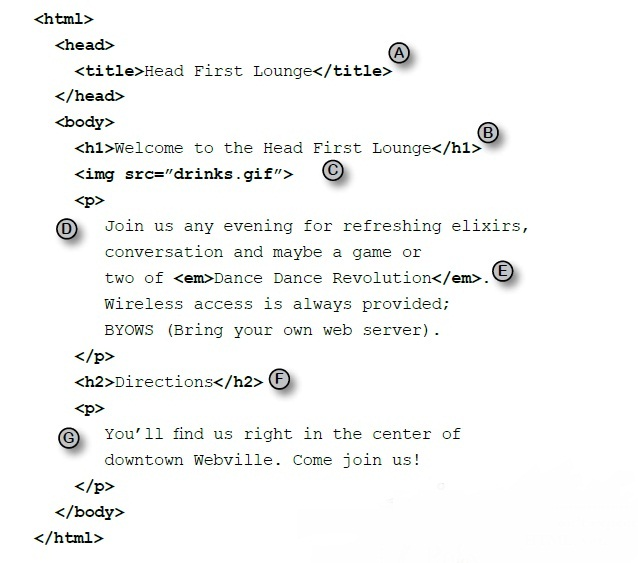
\includegraphics[width=0.7\textwidth]{img1.png}
\caption{Codigo HTML}
\label{fig:5.1}
\end{figure}

\singlespace
En la imagen (\ref{fig:5.2}) tambien observar la generacion del codigo al ser traducido por un navegador

\begin{figure}[htb]
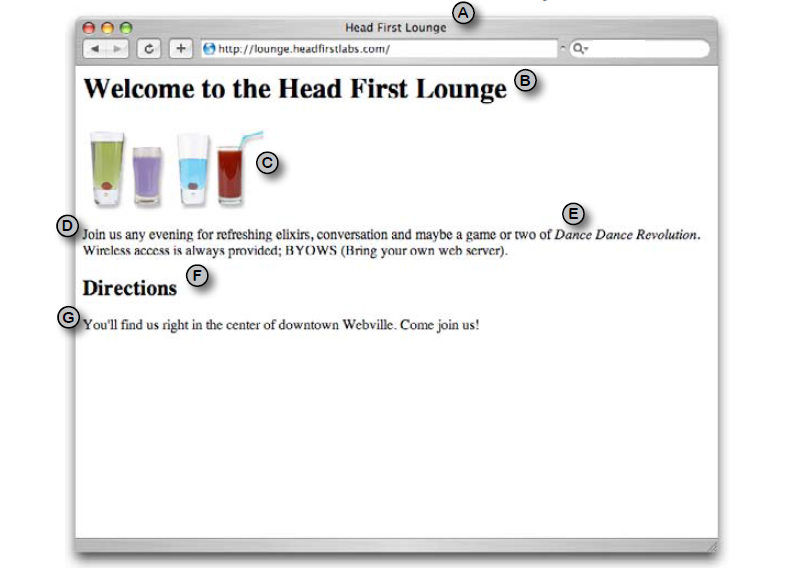
\includegraphics[width=0.7\textwidth]{img2.png}
\caption{Codigo HTML ejecutado por navegador}
\label{fig:5.2}
\end{figure}




\end{document}
